\documentclass{article}
\title{
    \LARGE Seminar Report 1 \\ Algorithms and Data Structures\\[0.2em]
}
\author{Varvara Aladyina}
\date{January 2026}

\usepackage{graphicx}
\graphicspath{{images/}}

\usepackage{siunitx}

% To properly align numbers on the decimal
\sisetup{round-mode=figures, round-precision=4}

\usepackage{booktabs}
\usepackage{array} % Package to define new column types
\usepackage{pgfplotstable}
\usepackage{filecontents}
\usepackage{tikz}
\pgfplotsset{compat=1.18}
\usepackage[margin=1in]{geometry}
\usepackage{float}
\usepackage[utf8]{inputenc}
\usepackage[english]{babel}
\usepackage[style=ieee]{biblatex}
\addbibresource{references/references.bib}
\usepackage{csquotes}
\usepackage{longtable}
\usepackage{booktabs}
\usepackage{booktabs} % For better lines in tables
\usepackage[utf8]{inputenc}
\usepackage{hyperref}
\hypersetup{
    colorlinks=true,
    linkcolor=black,
    filecolor=magenta,
    urlcolor=blue,
}
\usepackage{listings}
\usepackage{multirow, makecell}
\usepackage{pgfplots}
\pgfplotsset{compat=1.18}
\usepackage{caption}
\usepackage{calculator}
\usepackage{calculus}
\usepackage{adjustbox}
\usepackage{geometry}
\geometry{
    a4paper,
    left=30mm,
    right=30mm,
    top=25mm,
    bottom=30mm,
    headheight={90pt},
}
\usepackage[shortlabels]{enumitem}

\usepackage{enumitem}
\usepackage{tabularx}
\usepackage{booktabs}

\addto\captionsenglish{\renewcommand{\listfigurename}{Plots}}
\addto\captionsenglish{\renewcommand{\listtablename}{Tables}}

\begin{document}
\begin{figure}[ht!]
    \minipage{0.76\textwidth}
    
\includegraphics[width=7cm]{images/hkr.png}
    \label{title}
    \endminipage
    \minipage{0.32\textwidth}
    \endminipage
\end{figure}

\vspace{0.8cm}
\large

\textbf{{\let\newpage\relax\maketitle}}

\begin{center}
    \vfill
    \small{Kristianstad University | SE-291 88 Kristianstad | +46 44 250 30 00 | www.hkr.se}
\end{center}

\thispagestyle{empty}

\newpage

\makeatletter
\renewcommand{\abstractname}{\vspace{-\baselineskip}}
\begin{abstract}
    \large
    \noindent\textbf{Title}\\
    Seminar Report 1 Algorithms and Data Structures\\[1em]
    \textbf{Programme}\\
    Software Development\\[1em]
    \textbf{Author}\\
    Varvara Aladyina\\[1em]
    \textbf{Abstract}\\
     This report compares the performance of 2 sorting algorithms (Insertion Sort and Quick Sort) and measures effectiveness of Binary Search. Practical runtime measurements are compared to theoretical Big-O complexity. Results show Quick Sort outperforms Insertion Sort significantly. Binary Search times remain nearly constant across input sizes, matching its $O(log n)$ expectation\\[1em]
    \textbf{Keywords}\\
    Sorting algorithms, Algorithms, Measuring effectiveness, Big-O, Iterative vs Recursive \\[1em]
    
\end{abstract}
\makeatother

\newpage

\tableofcontents
\thispagestyle{empty}

\newpage
\section{Introduction}
This report describes results that were got from testing 3 algorithms: insertion sort, quick sort and binary search. A comparison between theretical and real results will be shown. The main goal is to understand how implementation style affects speed of the algorithms.
The following questions will be asked:
\begin{itemize}
    \item How effective are quick and insertion sort algorithms compared to each other?
    \item Is there a huge difference between iterative and recursive implementations of sorting algorithms?
    \item Does the real-world performance match the theoretical Big-O complexity?
\end{itemize}

\section{Methodology}
%The method part describes how the study was done, on what bases and what type of data was collected and how it was analysed.
%We are trying to look alike a short academic report and in that context a method is of high value. It shows what kind of study we did, what data we collected and how we went on with analysing it.
%Our "method" could roughly be defined as follows.
The report based both on analytical and practical methods.

\subsection{Analytical methods}
Before and after assignment, literature review was made on sorting algorithms, their various implementations and time complexities. Theoretical research helped to understand more about sorting and algorithms and their visualization. 

\subsection{Practical methods}
The following tools were used to generate objective quality metrics:
\begin{itemize}
    \item Algorithm code (iterative and recursive versions).
    \item Measuring function of time.
    \item Linux (Debian) computer for testing.
\end{itemize}
Implemented algorithms were completely written by Rust(v.1.92.0). It was chosen because of the wish to learn a new language. Measuring time of algorithms being calculated was done on linux computer with 8 GB RAM on one core(Intel i5-7400) only.
To run sorting algorithms, same unsorted data was used from text file that was provided from the teacher that had one million of numbers with range from 0 to 99. Algorithms were tested with different array sizes, such as 1.000, 2.500, 5.000, 7.500, 10.000,  25.000, 50.000, 75.000, 100.000, 250.000, 500.000, 750.000,  1.000.000. Those values were slices from original array. Code was ran 20 times to get the measurements. 

\section{Results}

\subsubsection{Sorting algorithms}

Folowing data shows objectively average(16) measured execution time of each of sorting algorithms across different input sizes. Time is written here in milliseconds.
\begin{table}[h!]
    \centering
    \caption{Sorting Algorithm Performance (1 to 75.000)}
    \begin{tabular}{|c|r|r|r|r|r|r|r|r|}
        \toprule
        Algorithm & 1000 & 2500 & 5000 & 7500 & 10000 & 25000 & 50000 & 75000 \\
        \midrule
        InsertSort (iter) & 0.9285 & 5.5912 & 22.0935 & 49.8668 & 88.3142 & 551.9875 & 2\,203.4824 & 4\,955.8139 \\
        InsertSort (rec)  & 0.9734 & 6.0680 & 24.0330 & 53.7502 & 94.9802 & 594.7616 & 2\,370.8271 & 5\,328.6976 \\
        QuickMedian (iter)& 0.0075 & 0.0044 & 0.0027 & 0.0029 & 0.0018 & 0.0029 & 0.0038 & 0.0045 \\
        QuickRandom (iter)& 0.0142 & 0.0050 & 0.0049 & 0.0048 & 0.0049 & 0.0063 & 0.0071 & 0.0071 \\
        QuickFirst (iter) & 0.0047 & 0.0035 & 0.0024 & 0.0020 & 0.0019 & 0.0023 & 0.0032 & 0.0038 \\
        QuickMedian (rec) & 0.0138 & 0.0306 & 0.0423 & 0.0474 & 0.1038 & 0.2748 & 0.4228 & 0.7057 \\
        QuickRandom (rec) & 0.0088 & 0.0204 & 0.0343 & 0.0626 & 0.0671 & 0.2282 & 0.3390 & 0.5431 \\
        QuickFirst (rec)  & 0.0084 & 0.0318 & 0.0652 & 0.0799 & 0.0841 & 0.2983 & 0.6652 & 0.8680 \\
        \bottomrule
    \end{tabular}
\end{table}

\begin{table}[h!]
    \centering
    \caption{Sorting Algorithm Performance (100.000 to 1.000.000)}
    \begin{tabular}{|c|r|r|r|r|r|}
        \toprule
        Algorithm & 100000 & 250000 & 500000 & 750000 & 1\,000\,000 \\
        \midrule
        InsertSort (iter) & 8\,805.4626 & 55\,062.4417 & 220\,160.6312 & 495\,403.7771 & 880\,939.3268 \\
        InsertSort (rec)  & 9\,466.1956 & 59\,164.0952 & 236\,605.2783 & 532\,373.3531 & 946\,771.7399 \\
        QuickMedian (iter)& 0.0051 & 0.0178 & 0.0317 & 0.0380 & 0.0471 \\
        QuickRandom (iter)& 0.0077 & 0.0141 & 0.0254 & 0.0322 & 0.0407 \\
        QuickFirst (iter) & 0.0044 & 0.0095 & 0.0182 & 0.0273 & 0.0371 \\
        QuickMedian (rec) & 0.8518 & 5.7651 & 5.2019 & 7.4712 & 10.1385 \\
        QuickRandom (rec) & 0.7443 & 1.5966 & 3.4505 & 5.6544 & 6.3810 \\
        QuickFirst (rec)  & 1.3767 & 2.8364 & 4.8917 & 9.0962 & 16.9172 \\
        \bottomrule
    \end{tabular}
\end{table}

\begin{figure}[htbp]
    \centering
    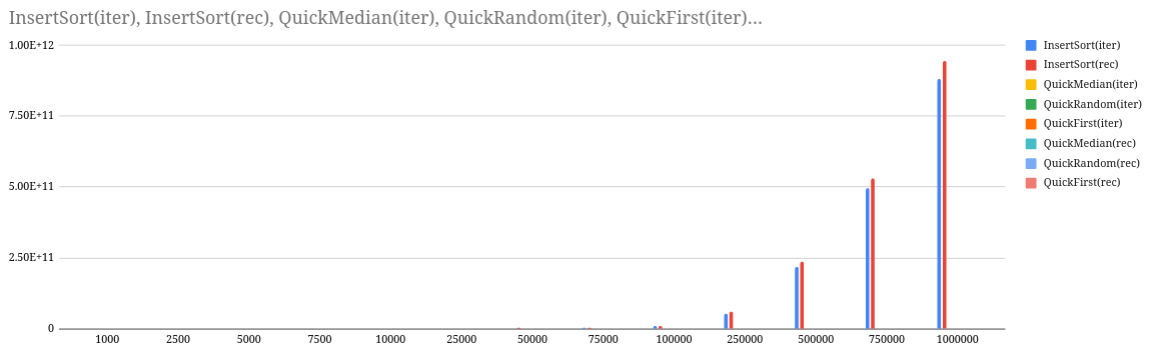
\includegraphics[width=\textwidth]{sort_chart.png}
    \caption{Chart of all sorting algorithms}
    \label{fig:my_label}
\end{figure}
\begin{figure}[htbp]
    \centering
    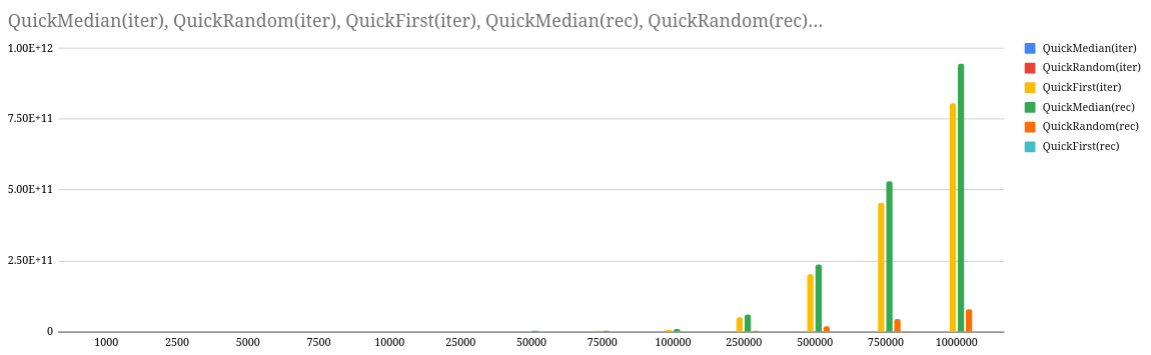
\includegraphics[width=\textwidth]{quick_chart.png}
    \caption{Chart of quick sorting algorithms}
    \label{fig:my_label}
\end{figure}

\newpage

\subsection{Binary search}
The average execution time for binary search (in nanoseconds) was calculated from 70 runs per input size. The target value was guaranteed to exist in the sorted array for each test. Sorted array was created by iteration that went from 1 up to 2.048.000.

\begin{table}[htbp]
    \centering
    \caption{Sorting Algorithm}
    \label{tab:sorting_horizontal}
    \begin{tabular}{|c|c|c|c|c|c|c|}
        \hline
        \textbf{Size} & 1k & 2k & 4k & 8k & 16k & 32k \\
        \hline
        \textbf{Time (ns)} & 45.91 & 38.61 & 35.55 & 35.93 & 36.18 & 35.95 \\
        \hline
        \textbf{Size} & 64k & 128k & 256k & 512k & 1024k & 2048k \\
        \hline
        \textbf{Time (ns)} & 35.85 & 50.96 & 37.74 & 36.81 & 35.68 & 38.39 \\
        \hline
    \end{tabular}
\end{table}
\newpage

\section{Discussion}
\subsection{Sorting algorithms}
\subsubsection{Insert sort}
From the figure 1 it is seen clearly that both insertion sort implementations take way more time than any of the quick sorts.This matches the theoretical expectation: insertion sort is $O(n^2)$, while quick sort is $O(n \log n)$ on average.

The recursive insertion sort was slower than the iterative one, probably because insertion sort is naturally iterative, and recursion adds extra function call overhead without any benefit.

\subsubsection{Quick sort}
On the figure 2 it is seen that iterative implementations are extremelly fast, often completing in less than 0.05 ms even for one million elements, meanwhile recursive implementation takes way more time. Among iterative versions, first pivot was often the fastest, while median pivot showed slightly more variability. For recursive implementations, random pivot with recursive implementation tended to be the most consistent, probably because of the average value. The median pivot with iterative implementation was sometimes slower than expected, which might be due to the extra computation needed to find the median.

\section{Summary}
This practical investigation confirmed several key points:
\begin{itemize}
\item Quick sort is dramatically faster than insertion sort for large datasets.
\item Iterative sorting algorithms tend to be quicker their recursive counterparts due to lower overhead.
\item The observed growth rates for insertion sort ($O(n^2)$), quick sort ($O(n \log n)$), and binary search ($O(\log n)$) align well with theoretical predictions.
\item Even within quick sort, pivot selection and iterative/recursive implementation cause measurable time differences.
\end{itemize}

%\section{Bibliography}
%\printbibliography[heading=none]

\end{document}

%https://coderscratchpad.com/rust-program-to-implement-binary-search/
%https://www.geeksforgeeks.org/dsa/iterative-quick-sort/
%https://www.geeksforgeeks.org/dsa/binary-search/
%
